\documentclass{beamer}
\usepackage{amsmath}
\usepackage{fourier}
\usetheme{metropolis}

\title{\vspace{-0.5cm}Parameter estimation\\of partial differential equations\\via neural networks}
\author{Alexander Glushko, Dmitry I.\ Kabanov}
\date{Final project on the Stochastic Numerics course\\Once upon a time in 2019}

\newcommand{\Data}{\vec{D}}
\newcommand{\DataExt}{\widetilde{\vec{D}}}
\newcommand{\MSE}{\ensuremath{\text{MSE}}}
\newcommand{\T}{\ensuremath{\text{T}}}
\renewcommand{\vec}[1]{\boldsymbol{#1}}
\newcommand{\VTheta}{\ensuremath{\vec{\theta}}}
\newcommand{\VLambda}{\ensuremath{\vec{\lambda}}}
\DeclareMathOperator*{\argmin}{arg\,min}
\newcommand{\R}{\mathbb R}
\newcommand{\UNN}[1][\text{NN}]{u_{#1}}
\newcommand{\FNN}[1][\text{NN}]{f_{#1}}
\newcommand{\NonlinOp}{\mathcal N\!}

\begin{document}
\maketitle

% ------------------------------------------------------------------------------
% Common part
\begin{frame}{Outline}
\begin{itemize}
    \item Introduction to the problem of parameter estimation of PDEs
    \item Solution set up
    \item Description of neural networks
\end{itemize}
\end{frame}

% Common part (end)
% ------------------------------------------------------------------------------

%slide 3
\begin{frame}{Introduction}

The main goal fo our project is:

Given data $\vec{D} = \{t_i, x_i, u_i\},`~i = 1, ..., N,$ observed from the solution of PDE of the form
\begin{equation}
    \label{eq:pde}
    u_t + \mathcal N\!(u; \VLambda) = 0,
\end{equation}
estimate $\VLambda$.

Here $u=u(x, t)$ is the solution of the equation,
$\NonlinOp(u; \VLambda)$ a nonlinear algebraic-differential operator,
$\VLambda$ the vector of unknown parameters.

\end{frame}

%slide 4
\begin{frame}

By Bayes' rule, the optimal value of $\VLambda$ is found through
maximization of the posterior distribution \cite{sivia2006data}
\begin{equation}
    \rho( \VLambda | \Data ) \propto
    \rho( \Data | \VLambda ) \times \rho( \VLambda ).
\end{equation}

Furthemore, we assume
\begin{equation}
    u_i = u(x_i, t_i; \VLambda) + \epsilon_i, \quad i=1, \dots, N,
\end{equation}
where $\epsilon_i \sim N(0, \sigma^2)$, and assign uninformative prior for $\VLambda$
\begin{equation}
    \rho(\vec{\lambda}) = \text{const} \quad \text{ for all } \vec{\lambda},
\end{equation}
so that, the problem of finding $\VLambda$ is a nonlinear unconstrained
optimization problem
\begin{equation}
    \label{eq:optim-ideal}
    \argmin_{\VLambda} \quad 
    \log \sum_{i=1}^{N} \big[ u_i - u(x_i, t_i; \VLambda) \big]^2,
\end{equation}
here noise variance $\sigma^2$ is a~
nuisance parameter~\cite[section~8.2]{sivia2006data}
    
\end{frame}

% slide 5
\begin{frame}

Analytical solution of the optimization problem~\eqref{eq:optim-ideal} can be expensive, so following \cite{raissi2017pinnII}.
we replace  $u(x_i, t_i; \VLambda)$ with a 
feedforward neural network \cite{goodfellow2016deep}
\begin{equation}
\UNN(x, t; \vec{\theta}) = g_L \circ g_{L-1} \circ \dots \circ g_1,
\end{equation}
where
\[
    g_\ell(z; \VTheta_\ell) = \sigma (W_\ell z + b_\ell), \quad \ell = 1,\dots,L,
\]
with $L$ is the number of layers in the network, with layers 0 and $L$ being
input and output layers, respectively, and layers from 1 to $L-1$ being hidden
layers, $\sigma$ being a nonlinear activation function applied
componentwise. In this work, we plan to use \( \sigma(z) = \tanh (z) \).
    
\end{frame}

%slide 6
\begin{frame}
    
\end{frame}

% ------------------------------------------------------------------------------
% Heat equation part



% Heat equation part (end)
% ------------------------------------------------------------------------------

% ------------------------------------------------------------------------------
% Burgers' equation

\section{Burgers' equation}

%slide 1
\begin{frame}

Let us consider the Burgers' equation. This equation is nonlinear and serves as a prototype of the governing equations of fluid dynamics [1]. 
\begin{equation}
    \frac{\partial u}{\partial t} + u \frac{\partial u}{\partial x} = \nu^2 \frac{\partial^2 u}{\partial x^2}
\end{equation}
For small values of the viscosity parameter $\nu$ , Burgers' equation can lead to shock formation that is notoriously hard to resolve by classical numerical methods. 

\end{frame}

% silde 2
\begin{frame}
In this project we are going to consider the input data of the following form of the Burgers' equation:
\begin{align}

u_t + u u_x - (0.01/\pi)u_{xx} = 0, x \in [-1, 1], t \in [0, T], &\\
u(0, x) = -sin(\pi x), & \\
u(t, -1) = u(t, 1) = 0.
\end{align}
As we are solving the inverse problem, our goal is to find values:
$$\lambda_1 = 1, ~ \lambda_2 = (0.01 / \pi) \approx 0.318, $$ using the following input data matrices:
$t \in [0, 1] \text{ of size } [100, 1], \\ ~ x \in [-1, 1] \text{ of size } [256, 1],~ u \text{ of size } [256, 100].$

\end{frame}

% slide 3
\begin{frame}

Optimising all loss functions using L-BFGS (a quasi-Newton, full-batch gradient-based optimisation algorithm [2]), we have got the following bootstrapped results:

\begin{center}
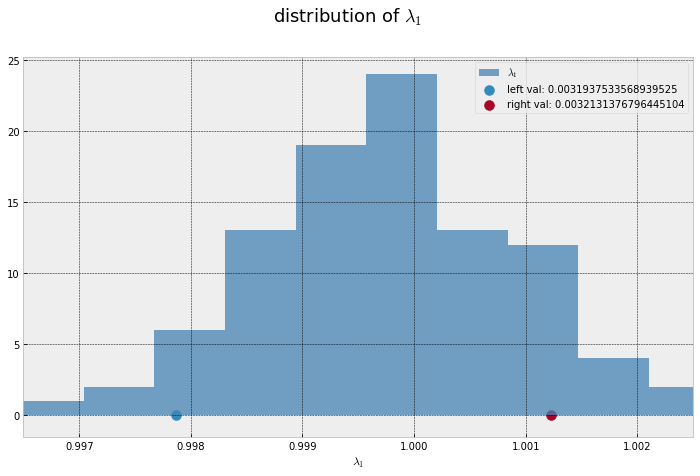
\includegraphics[width = 5.7cm , height = 4cm]{02-presentation-v1/images/l1_confidence.png}
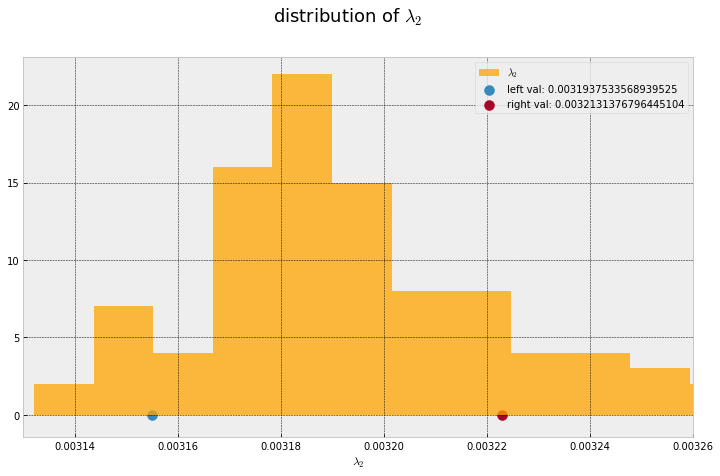
\includegraphics[width = 5.7cm , height = 4cm]{02-presentation-v1/images/l2_confidence.png}
\\
\caption{Figure 1. Bootstrapped parameters $\lambda_1$ and $\lambda_2$ for Burgers' equation.}
\end{center}
\end{frame}

% slide 4
\begin{frame}

The panel of Figure 2 shows the predicted spatio-temporal solution u(t,x), along with the locations of the initial and boundary training data. This prediction is obtained without any sort of discretization of the spatio-temporal domain. 

\begin{center}
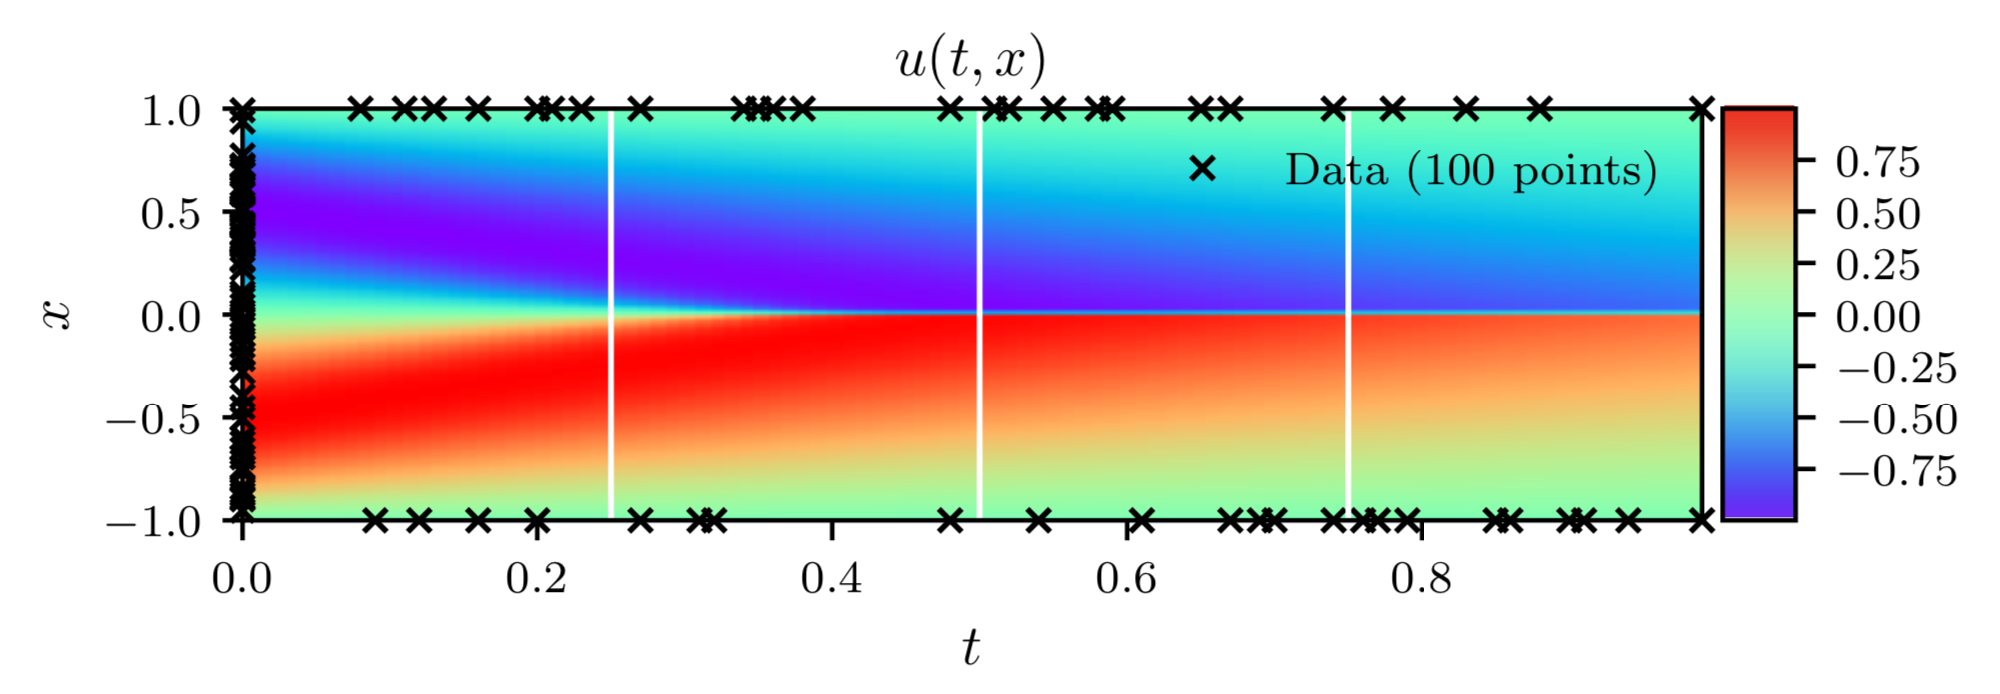
\includegraphics[width = 10cm , height = 4cm]{02-presentation-v1/images/predicted_sol_burgers.png}
\\
\caption{Figure 2. Predicted solution $u(t,x)$ along with the initial and boundary training data.}
\end{center}

\end{frame}

% slide 5
\begin{frame}

Below, we present a comparison between the exact and the predicted solutions at different time instants t = 0.25, 0.50, 0.75. The physics informed NN accurately captures the nonlinear behavior of the Burgers' equation that leads to the development of a sharp internal layer around t = 0.4.
    
\begin{center}
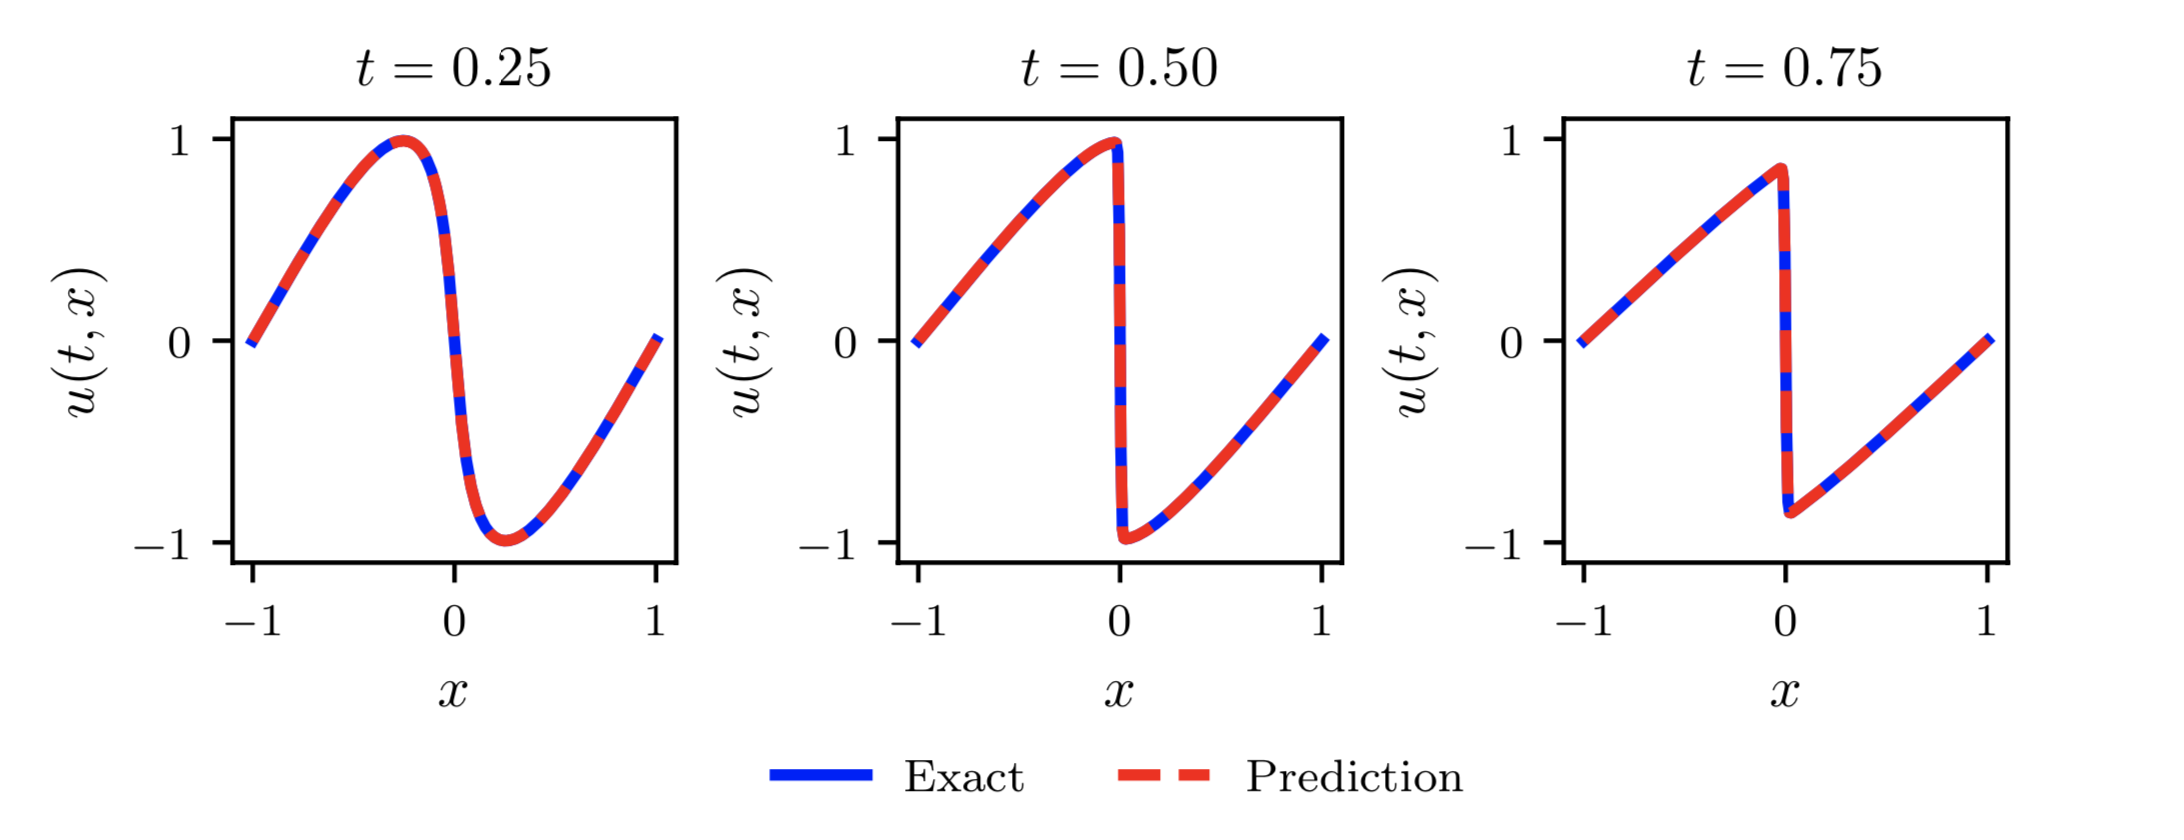
\includegraphics[width = 8cm , height = 4cm]{02-presentation-v1/images/exact_pred_burgers.png}
\\
\caption{Figure 3. Comparison of the predicted and exact solutions corresponding to the three temporal snapshots depicted by the white vertical lines in the top panel.}
\end{center}

\end{frame}

% slide 6
\begin{frame}

Therefore, a key property of physics informed neural networks is that they can be effectively trained using small data sets; a setting often encountered in the study of physical systems for which the cost of data acquisition may be prohibitive.
    
\end{frame}

%slide 7
\begin{frame}{Reference}

[1] C. Basdevant, M. Deville, P. Haldenwang, J. Lacroix, J. Ouazzani, R. Peyret, P. Orlandi, A. Patera, Spectral and finite difference solutions of the Burgers equation, Computers & fluids 14 (1986) 23 - 41.

[2] D. C. Liu, J. Nocedal, On the limited memory BFGS method for large scale optimization, Mathematical programming 45 (1989) 503–528. 

\end{frame}

% Burgers' equation (end)
% ------------------------------------------------------------------------------

\begin{frame}
    \frametitle{Conclusions}

\end{frame}


\bibliography{presentation}
\bibliographystyle{abbrv}

\end{document}
